\mainmatter
\pagestyle{headings}

\chapter{Methodology}
\label{ch:methodology}
\section{Research Questions \& Hypotheses}
To determine the influence of chatbots on the telecom industry, various questions must be asked of the industry's participants.\\
\break
\textbf{Main Question: What is the influence of customer service chatbots for both the customer experience and the business value?}\\
\break 
Three research questions were formulated to answer this main research question:

\subsubsection{RQ1: Are current chatbots effective in helping people and solving their problems?}
It is illogical to think that there will be people who will keep a good impression of a chatbot after it was unable to help with or solve their existing problem. Multiple studies suggest that it is essential that the execution done by a chatbot is effective \citep*{Muizzah2021, Brandtzaeg2018}.\
In a task-oriented chatbot, under which a chatbot can be placed, usefulness is key \citep{brandtzaeg2020}. Solving problems and providing help in an effective and efficient manner is the key to providing a good user experience. It is also crucial that the user's intentions are correctly interpreted and answered adequately.\\
\break
\citeauthor{Verkeyn2018} categorized 28 quality attributes and divided them up in 5 dimensions. Based on these quality attributes, the evaluation of a chatbot is possible (see \ref{ch:literature-study}. Literature Study). Relevant quality attributes that can be linked to the research question serve as the foundation for the hypotheses.\\
\break
\break
Related hypotheses:
\begin{enumerate}
	\setlength\itemsep{-0.1em}
	\item H1: Current chatbots execute requested tasks correctly. Based on \citeauthor{Verkeyn2018} quality attribute “Execute requested tasks” from the dimension “Functionality” (\acrshort{qa} 1).
	\item H2: Current chatbots can deliver the same services as a human agent. Based on \citeauthor{Verkeyn2018} quality attribute “Number of services available in the chatbot” from the dimension “Functionality” (\acrshort{qa} 2).
	\item H3: Current chatbots contain enough knowledge to provide good assistance. Based on \citeauthor{Verkeyn2018} quality attribute “Contains breadth of knowledge” from the dimension “Trustworthiness” (\acrshort{qa} 3).
\end{enumerate}

\subsubsection{RQ2: Are current chatbots easy to use and accessible?}
When a chatbot is effective in helping people, but is so complex or unusable that nobody uses it again, it is rational to assume that this chatbot has not made a good impression. In addition, a chatbot should be easily accessible, so that a high level of service is always present.\\
\break
\break
Related hypotheses:
\begin{enumerate}
	\setlength\itemsep{-0.1em}
	\item H4: Current  chatbots are easy to use. Based on \citeauthor{Verkeyn2018} quality attribute “Ease of use” from the dimension “Efficiency” (\acrshort{qa} 4).
	\item H5: Current  chatbots are available at all times (24/7). Based on \citeauthor{Verkeyn2018} quality attribute “Available at all times” from the dimension “Efficiency” (\acrshort{qa} 5).
\end{enumerate}

\subsubsection{RQ3: Do current chatbots create a pleasant customer experience?}
When a customer uses a service or buys a product from a company, it is important that the customer has a good feeling about how this interaction went.\\
\break
A “pleasant” customer experience can be seen as an experience where the customer is helped in a friendly and smooth way. It is not about the effectiveness or ease-of-use, although these have an impact on the experience as well. \\
\break
\break
Related hypotheses:
\begin{enumerate}
	\setlength\itemsep{-0.1em}
	\item H6: Current chatbots create an enjoyable interaction. Based on \citeauthor{Verkeyn2018} quality attribute “Create an enjoyable interaction” from the dimension “Humanity” \citep{Morrissey2013} (\acrshort{qa} 6).
\end{enumerate}

\section{Methodology - Business Interviews}
To gain more insight into what the chatbot means for telecom businesses, an exploratory research was conducted through interviews. The interviews were conducted with conversational designers, product owners, developers and AI trainers from Proximus, Telenet, T-Mobile and KPN. The write-outs of these interviews can be found in the \ref{ch:appendices}ppendices. The interview consists of four main parts:

\subsection{The current state of the chatbot}
The chatbot's general specifications were questioned in the first phase, this can be explained in terms of the capabilities (FAQs, complaint handling, sales, etc. ), the platforms on which the bot can be found, the languages in which it can be used, the age group of the relevant users, and the types of questions the bot can answer (yes/no questions, open/vague questions).

\subsection{The benefits that the company derives from the presence of the chatbot}
This section focuses on the benefits that the firm receives from using the chatbot. For example, the chatbot is asked what services it can provide. This pertains to renewing or forming a new membership, purchasing products/services, obtaining specific invoice details, and so on. The question also asks to what extent the chatbot can reduce customer support workload, and then goes into further depth about how many questions or tasks a chatbot cannot perform on its own. Furthermore, the focus is on how eager clients of the providers are to use a chatbot. Finally, the negative aspects of the story are discussed.

\subsection{The business value (revenue, reduced costs) realised by the chatbot}
The third part is about the business value that is created. First, it looks at how much extra direct turnover is created by the chatbot. Then it looks at how this value is generated, it asks about the availability of the chatbot, and how it handles conversations when no human agents are present. Next, it looks at what the initial strategic goal of the chatbot was, was it just added to improve customer service, or was it more of a marketing stunt?  It also asks how much the chatbot costs and which cost items were the most important. Finally, it looks at how many fewer people are employed in customer service because of the chatbot.

\subsection{The company's future vision of the chatbot}
The fourth and final part focuses on the company's future vision of the chatbot. They look at the extra features they want to add and how they want to improve the chatbot in terms of technology. Finally, they are asked how they determine what scenarios/dialogs they want to put in the bot and how they will apply this in the future.

\section{Methodology - Survey}
The research questions and hypotheses will be investigated by means of a joint survey.\\
\break
The joint survey in combination with the interviews will be used to generate the most amount of business value possible. For the business, the value is created by comparing the competition and gathering insight into what the customers consider important. For the customer, the value is found in better chatbots as a result of the study.\\

\subsection{Are these attributes present for the specific chatbot?}
To find out if the selected attributes are present, several questions will be used to check with the clients using the chatbots. The used questions per hypothesis are listed below.

\begin{longtable}{|l|l|}
	\hline
	\textbf{H1} & Did the chatbot fulfil your task correctly?                         \\ \hline
	\endfirsthead
	%
	\endhead
	%
	\textbf{H2} & Does the chatbot deliver the same services as a human?              \\ \hline
	\textbf{H3} & Did the chatbot contain enough knowledge to help with your problem? \\ \hline
	\textbf{H4} & Was the chatbot easy to use?                                        \\ \hline
	\textbf{H5} & Is the chatbot available at all times?                              \\ \hline
	\textbf{H6} & Did you enjoy interacting with the chatbot?                         \\ \hline
	\caption{An overview of each hypothesis along with its respective question.}
	\label{tab:YNOverview}
\end{longtable}
\ul{Rating scale}\\
For answering the statements, yes/no questions will be used to check the presence of these attributes.

\subsubsection{Data Evaluation Method - Comparative Study}
The chatbots will be compared to one another to see which attributes are present in which chatbot.

\subsection{How important are these attributes for the clients?}
The research questions and hypotheses will be investigated/evaluated by means of the proven KANO method. The method of application is inspired by the study of \citeauthor{Verkeyn2018}.\\
\break
To find out which of the chosen 6 attributes types are seen as important, the following questions per category will be used.

\begin{longtable}{|l|l|}
	\hline
	\textbf{H1} & The chatbot (DOES NOT) execute(s) the given task correctly           \\ \hline
	\endfirsthead
	%
	\endhead
	%
	\textbf{H2} & Does the chatbot deliver the same services as a human?               \\ \hline
	\textbf{H3} &
	\begin{tabular}[c]{@{}l@{}}The chatbot knows at least as much as an expert in the same\\ industry. / The chatbot knows less than an expert in\\ the same industry\end{tabular} \\ \hline
	\textbf{H4} & The chatbot is (NOT) easy to use.                                    \\ \hline
	\textbf{H5} & The chatbot is (NOT) available at all times.                         \\ \hline
	\textbf{H6} & The chatbot (DOES NOT) communicate(s) in a robotic, non-empathic way \\ \hline
	\caption{An overview of each hypothesis along with its respective KANO question.}
	\label{tab:KANOQuestions}
\end{longtable}
\ul{Rating scale}\\
For answering the statements, a five-level rating scale based on \citep{KANO1984}, will be used.\\
\break
The levels are as follows:
\begin{enumerate}
	\setlength\itemsep{-0.1em}
	\item I dislike it
	\item I can live with it
	\item I am neutral
	\item I expect it
	\item I like it
\end{enumerate}
This scale allows users to express how important a statement is.

\subsubsection{Data Evaluation Method - Comparative Study}
To be able to answer the second main question, there is a need for an evaluation method that will list the general user importance for each quality attribute. KANO is a tool that can satisfy these desires. The KANO Model gives more insight into the fact that the performance of the quality attributes is not in a linear relationship with the corresponding customer satisfaction \citep{KANO1984}. KANO offers the possibility to divide the quality attributes into five categories that each have different effects on customer satisfaction (Attractive, Performance, Must-Be, Indifferent, Reverse). This division is done on the basis of the answers obtained from the survey (questions with five-level rating scale).\\

\begin{figure}[ht]
	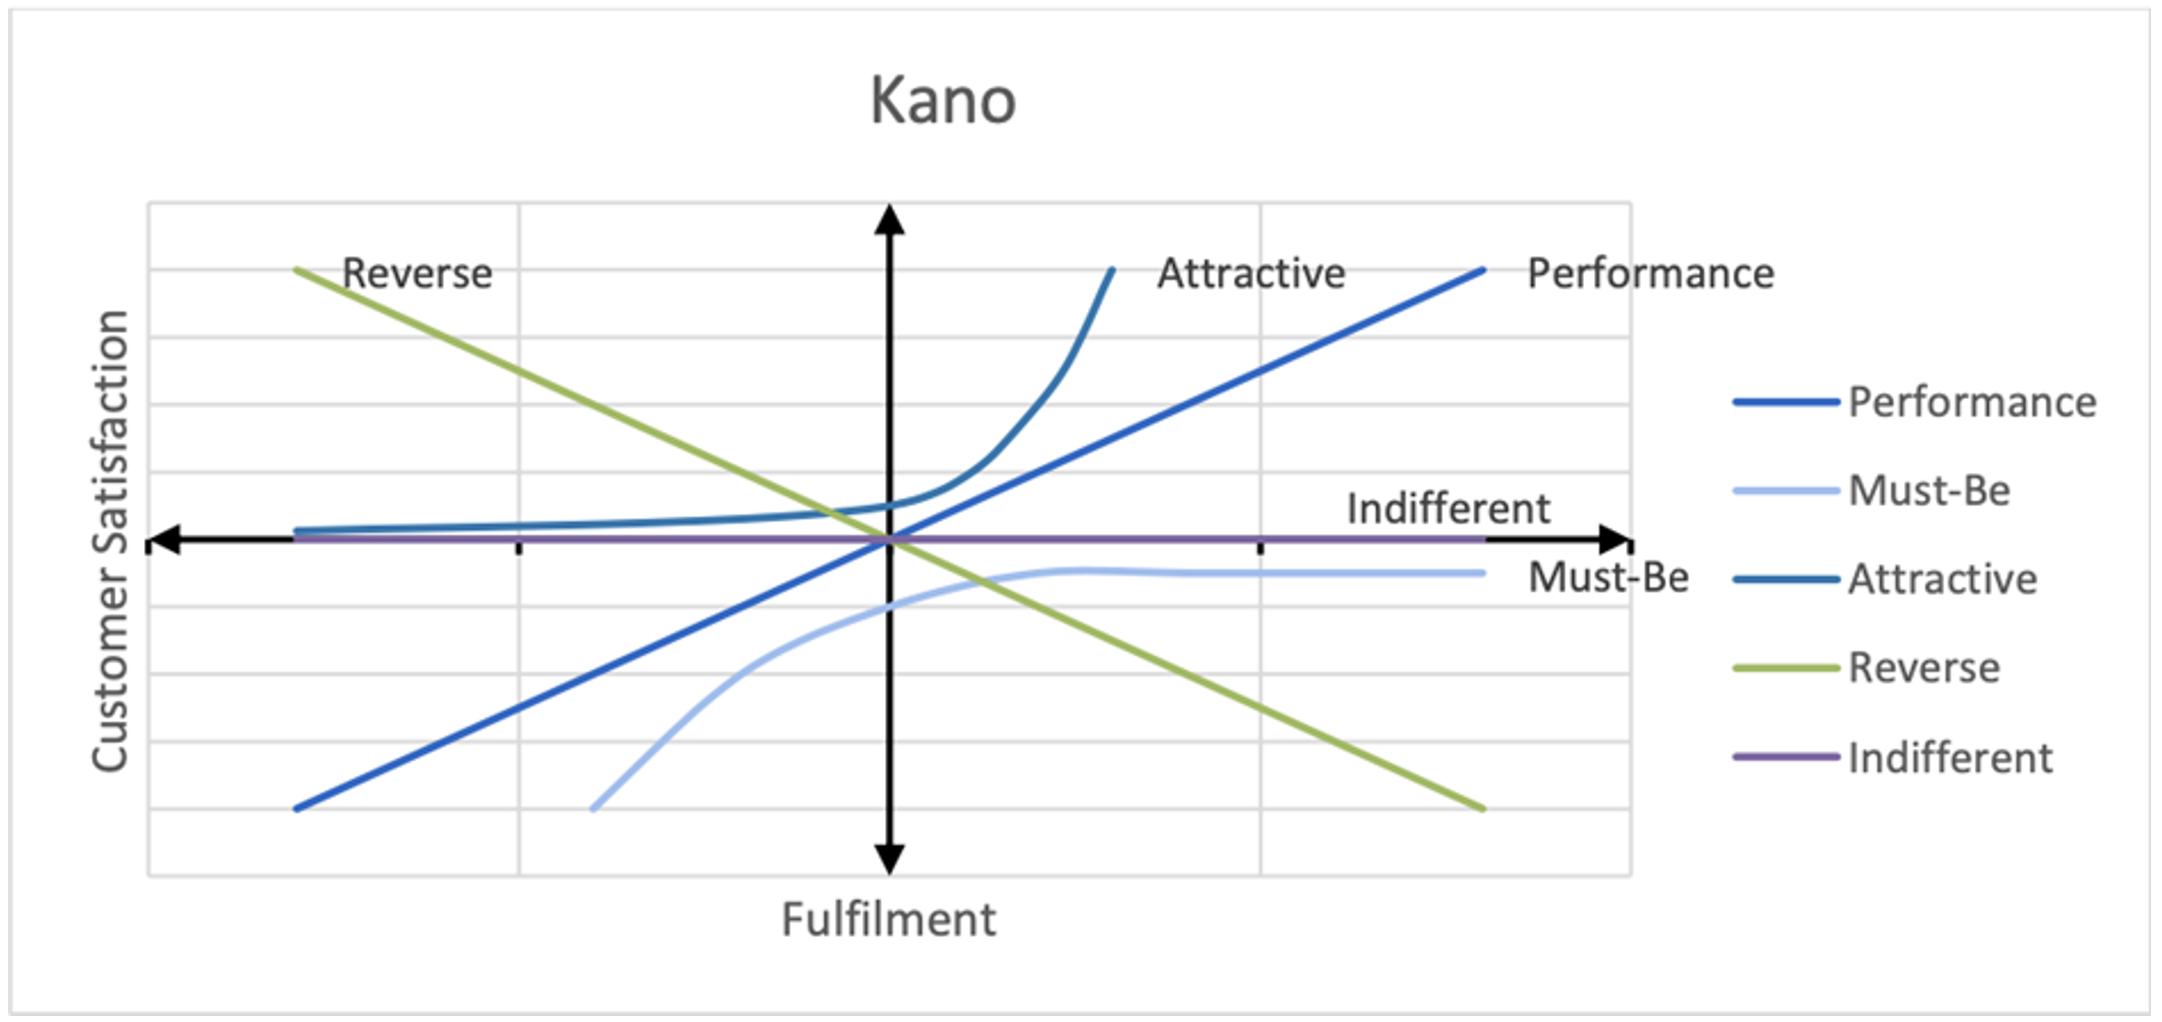
\includegraphics[scale=0.35]{../LaTeX/Figures/KANO.png}
	\caption{Five categories of quality attributes \citep{KANO1984}.}
	\label{fig:kano}
\end{figure}
\break
The five categories are represented visually as in Figure \ref{fig:kano}, each category showing a different relationship.\\
\break
Attractive: if a quality attribute from this category is more present, the customer satisfaction will increase more than linearly. When the quality attribute is not present, the customer will have neither a positive nor negative customer satisfaction.\\
\break
Performance: When a quality attribute from this category is present, the customer satisfaction will increase linearly. If the quality attribute is not present, then this will result in a negative customer satisfaction.\\
\break
Indifferent: If a quality attribute from this category is present, then this has no effect on customer satisfaction.\\
\break
Must-Be: The customer considers this kind of quality attribute as necessary, when it is not present, the customer satisfaction will be drastically low and the product basically has failed at this point.\\
\break
Reverse: The more these quality attributes are present, the worse the customer satisfaction. The customer satisfaction increases when they are less present.

\subsection{Survey arrangement}
The survey is divided up into 3 parts:\\
\break
\ul{Part 1 - general information about the participant and information on the interaction with the chatbot}\\
\break
In the first part, general information about the participant is requested such as the postal code, age, highest obtained degree, and gender, these variables can be added as control variables in the static models to process the results.\\
\break
Next, they are asked from which company they used the chatbot, what task they performed, in what language they addressed the chatbot and on what platform.\\
\break
\ul{Part 2 - questions about the interaction with the chatbot}\\
\break
The second part focuses on the interaction with the chatbot, the questions that were drawn up for the hypotheses in section \textbf{3.3.1 of the Methodology} are asked here. The results of this study are used to evaluate each company's chatbot, then a comparative study is conducted.\\
\break
\ul{Part 3 - questions about the customer expectations of a telecom customer service chatbot}\\
\break
The final part of the survey asks what the customer expects from customer service chatbot in various scenarios. In order to put the participant in a certain context, three different scenarios were created in which a customer might find himself with the corresponding telecom services. The three scenarios are as follows:
\begin{enumerate}
	\item You have not switched off your phone in a while and it  ran out of battery. You have a problem because you do not remember your PIN code. You ask the chatbot if he can retrieve your PIN code given your client details. 
	\item You are not happy with your subscription because it does not match your needs, from a friend you have heard there is a better deal so you want the chatbot to stop your subscription.
	\item At least once each month, you lose internet connectivity. You are tired of these problems and you want to file a complaint. You turn to the chatbot of your telecom provider with your complaint.
\end{enumerate}
After a participant is introduced to each scenario, they were asked each time to give their opinion on the statements drawn up in \textbf{3.3.2 of the Methodology}.

\subsection{Target group}
The target group of the survey will not be filtered on human characteristics, but it will be screened on whether the person has already had an experience with a telecom chatbot of a provider located in Belgium or in the Netherlands.
